% !TEX program = xelatex
% EECS 245: Mathematics for Machine Learning, Spring 2026 Midterm 1
% Compile with XeLaTeX or LuaLaTeX to use Avenir
\documentclass[11pt]{article}
\usepackage{../../eecs245}

% Uncomment the line below to show solutions in gray boxes
% \enablesolutions

% Uncomment the line below to include student name/uniqname section
\enablestudentinfo

% Enable exam mode to include UMID and room options
\enableexam

\usepackage{amsmath, amsfonts, amssymb, multicol, hyperref}
% Restore Computer Modern for math
\DeclareSymbolFont{operators}{OT1}{cmr}{m}{n}
\DeclareSymbolFont{letters}{OML}{cmm}{m}{it}
\DeclareSymbolFont{symbols}{OMS}{cmsy}{m}{n}

% Keep the exam uniqname header compact; the shared style's flushright header
% triggers large fancyhdr headheight warnings on odd pages.
\setlength{\headheight}{14pt}
\renewcommand{\examuniqnameheader}{%
  \ifnum\value{page}>2\relax
    \ifodd\value{page}%
      \makebox[0pt][r]{\textbf{uniqname:} \rule{5cm}{0.4pt}}%
    \fi
  \fi
}

% Metadata
\newcommand{\coursename}{EECS 245}
\newcommand{\term}{Spring 2026 at the University of Michigan}
\newcommand{\assignment}{Midterm 1}
\newcommand{\duedate}{}
\newcommand{\submissioninstructions}{

\textbf{Instructions}

\begin{itemize}
\item This exam consists of 9 problems, worth 100 points, spread across 12 pages (6 sheets of paper).
\item You have 120 minutes to complete this exam, unless you have extended-time accommodations through SSD.
\item Write your uniqname in the top right corner of each page.
\item For free response problems, \textbf{you must show all of your work}, and $\boxed{\text{circle}}$ your final answer. We will not grade work that appears elsewhere, and you may lose points if your work is not shown.
\item For multiple choice problems, completely fill in bubbles and square boxes; if we cannot tell which option(s) you selected, you may lose points. \\
\bubble{A bubble means that you should only select one choice.}  \\
\squarebubble{A square box means that you should select all that apply.}
\item You may refer to \textbf{one double-sided 8.5x11'' handwritten notes sheet}. Other than that, you may not refer to any other resources or technology during the exam (no phones, watches, or calculators).
\end{itemize}

}

\begin{document}
\makemytitle{\coursename}{\term}{\assignment}{}
{\submissioninstructions}
{\bubble{1690 BBB (1-3PM)} \bubble{1690 BBB (extended time)}}

\vspace{1em}

You are to abide by the University of Michigan/Engineering Honor Code. To receive a grade,
please sign below to signify that you have kept the Honor Code pledge.

\textit{I have neither given nor received aid on this exam, nor have I concealed any violations of the Honor Code.}

\emptybox{1.5cm}

\newpage

\begin{center}

\:

\vspace{9cm}
This page has been intentionally left blank.

\end{center}

\newpage

\textbf{Tip: Skim through the entire exam before starting to work on it.}

\begin{prob}[(16 pts)]
Suppose we'd like to find the optimal parameter, $w^*$, for the constant model
$h(x_i)=w$, using the following dataset of $n = 4$ values, $y_1, y_2, y_3, y_4$:
$$0, \quad 2, \quad 4, \quad 20$$

\begin{subprob}(3 pts) First, suppose we find the optimal parameter by minimizing mean squared error, $R_\text{sq}(w)$. Which value of $w$ minimizes $R_\text{sq}(w)$? Give your answer as a number with no variables. \\

$\text{minimizer of } R_\text{sq}(w) = \minibox{3cm}{13/2 = 6.5}[1cm]$

\begin{solution}
For the constant model, average squared loss is minimized at the mean of the $y_i$'s. Here,
\[
\frac{0+2+4+20}{4}=\frac{26}{4}=\boxed{\frac{13}{2}}
\]
\end{solution}
\end{subprob}


% . We are given a dataset of $n=4$ $y$-values:
% \begin{center}
% \begin{tabular}{c|c|c|c}
% $y_1$ & $y_2$ & $y_3$ & $y_4$ \\
% \hline
% 0 & 2 & 4 & 20 \\
% \end{tabular}
% \end{center}

Now, consider the \textbf{clipped} loss function, defined below. $$\displaystyle L_\text{clip}(y_i,h(x_i))=\min\{(y_i-h(x_i))^2,9\}$$
For example, $L_\text{clip}(10, 5) = 9$ and $L_\text{clip}(5, 3) = 4$.

Let $R_\text{clip}(w)$ be the average clipped loss for the constant model and this dataset.

\begin{subprob}(3 pts) State one value of $w$ where the derivative of $R_\text{clip}(w)$ is not defined. \\
$\text{one value of } w \text{ where the derivative of } R_\text{clip}(w) \text{ is not defined} =$ \minibox{3cm}{17}[1cm]
\begin{solution}
The clipped loss changes formulas whenever
\[
(y_i-w)^2=9
\]
Equivalently, this happens when $w=y_i\pm 3$. Since $20-3=17$, one valid answer is $\boxed{17}$.

For context, here's what average clipped loss looks like for this dataset: \\

\begin{center}
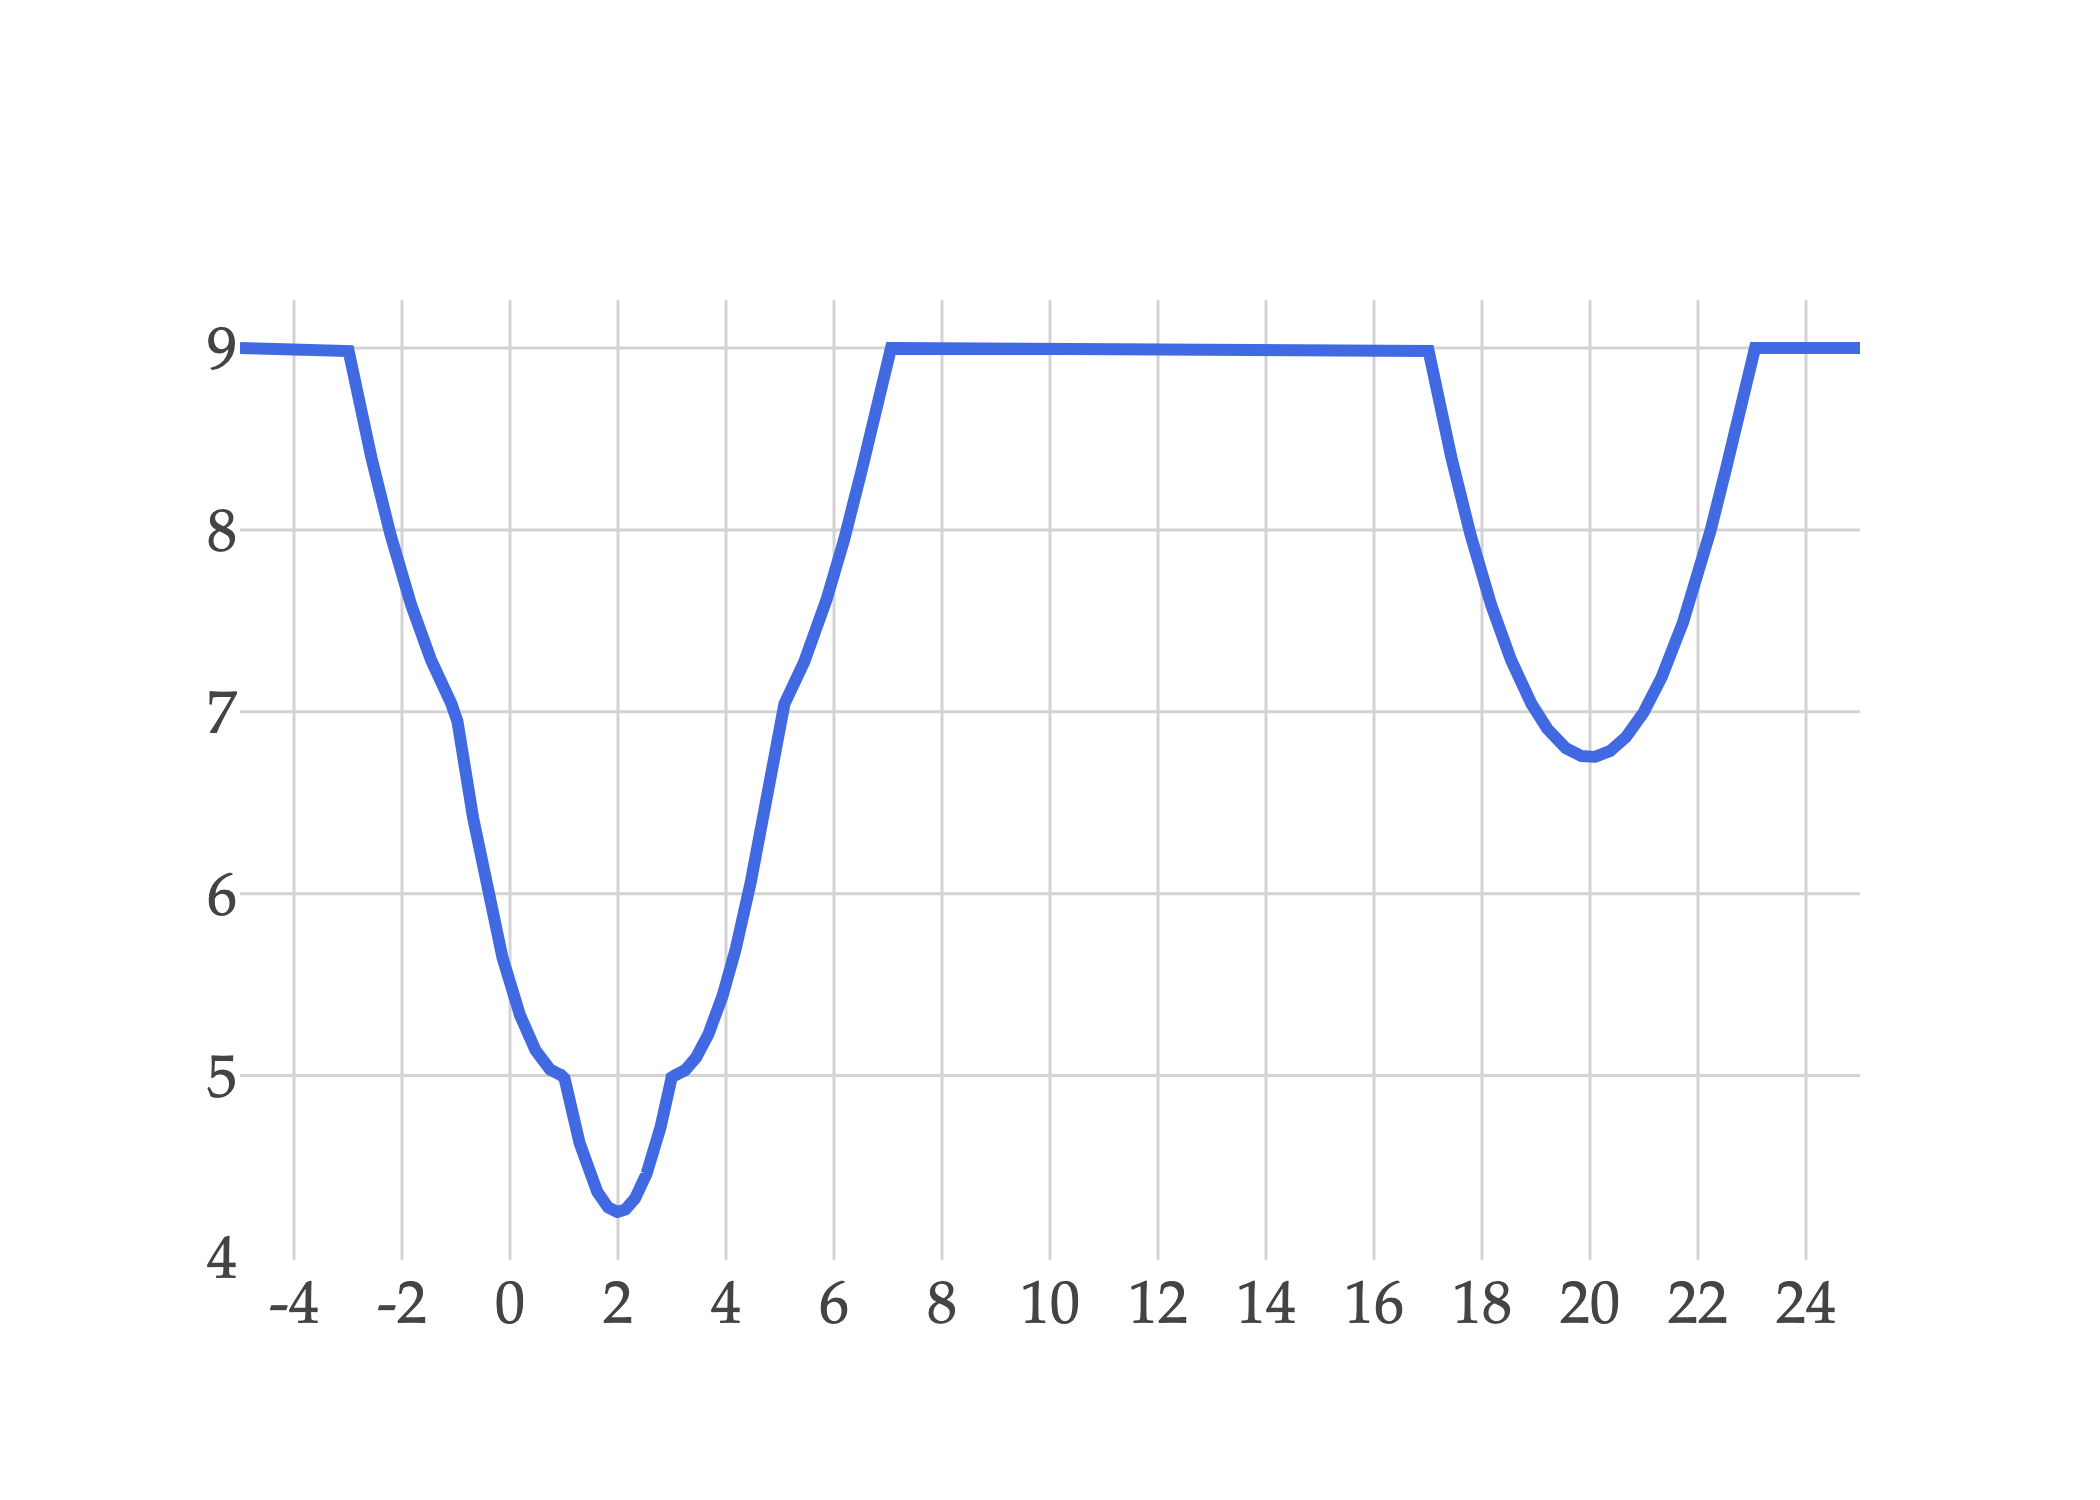
\includegraphics[width=0.9\textwidth]{imgs/p1-sol.png}
\end{center}
\end{solution}
\end{subprob}

\begin{subprob}(3 pts) Suppose we restrict $w$ to the interval $1 \leq w \leq 3$. Among all values of $w$ in this interval, which value minimizes $R_\text{clip}(w)$? Give your answer as a number with no variables. \\

$\text{minimizer of } R_\text{clip}(w) \text{ within the interval } [1, 3] = \minibox{3cm}{2}[1cm]$
\begin{solution}
Once $w$ is more than 3 units away from any particular $y_i$ value, the value $(y_i - w)^2$ is replaced by the constant $9$ when computing average loss. \\

What do we know about constants when they are added to functions? \textbf{They don't affect the minimizer!} That is, the minimizer of $f(x)$ and of $f(x) + c$ are the same. \\

What this is saying is that if $w$ is restricted to the interval $1 \leq w \leq 3$, we can ignore $y_4 = 20$ when computing the minimizer, and this just reduces to minimizing average squared loss (mean squared error) across the data points that are within 3 units of $w$. As long as $1 \leq w \leq 3$, we are within 3 units of $y_1 = 0$, $y_2 = 2$, and $y_3 = 4$. \\

What constant minimizes average squared loss, for the dataset $0, 2, 4$? That's the mean of $0, 2, 4$, which is $2$. So the minimizer of $R_\text{clip}(w)$ within the interval $1 \leq w \leq 3$ is $\boxed{2}$. \\

If you'd like to see this a little more formally, then when $1 \leq w \leq 3$,
\[
R_\text{clip}(w)=\frac14\left(w^2+(2-w)^2+(4-w)^2+9\right)
\]
Taking the derivative,
\[
\frac{\text{d}}{\text{d}w}R_\text{clip}(w)=\frac14(2w+2(w-2)+2(w-4))=\frac{6w-12}{4}
\]
Setting this equal to $0$ gives $w = 2$, as we intuited earlier.
\end{solution}
\end{subprob}

\begin{subprob}(3 pts) Now suppose there are no restrictions on $w$. Among all possible values of $w$, which value minimizes $R_\text{clip}(w)$? Give your answer as a number with no variables. \\

$\text{minimizer of } R_\text{clip}(w) = \minibox{3cm}{2}[1cm]$
\begin{solution}
The best $w$ is still $w = 2$. As a refresher, let's look at the graph of $R_\text{clip}(w)$ again: \\
\begin{center}
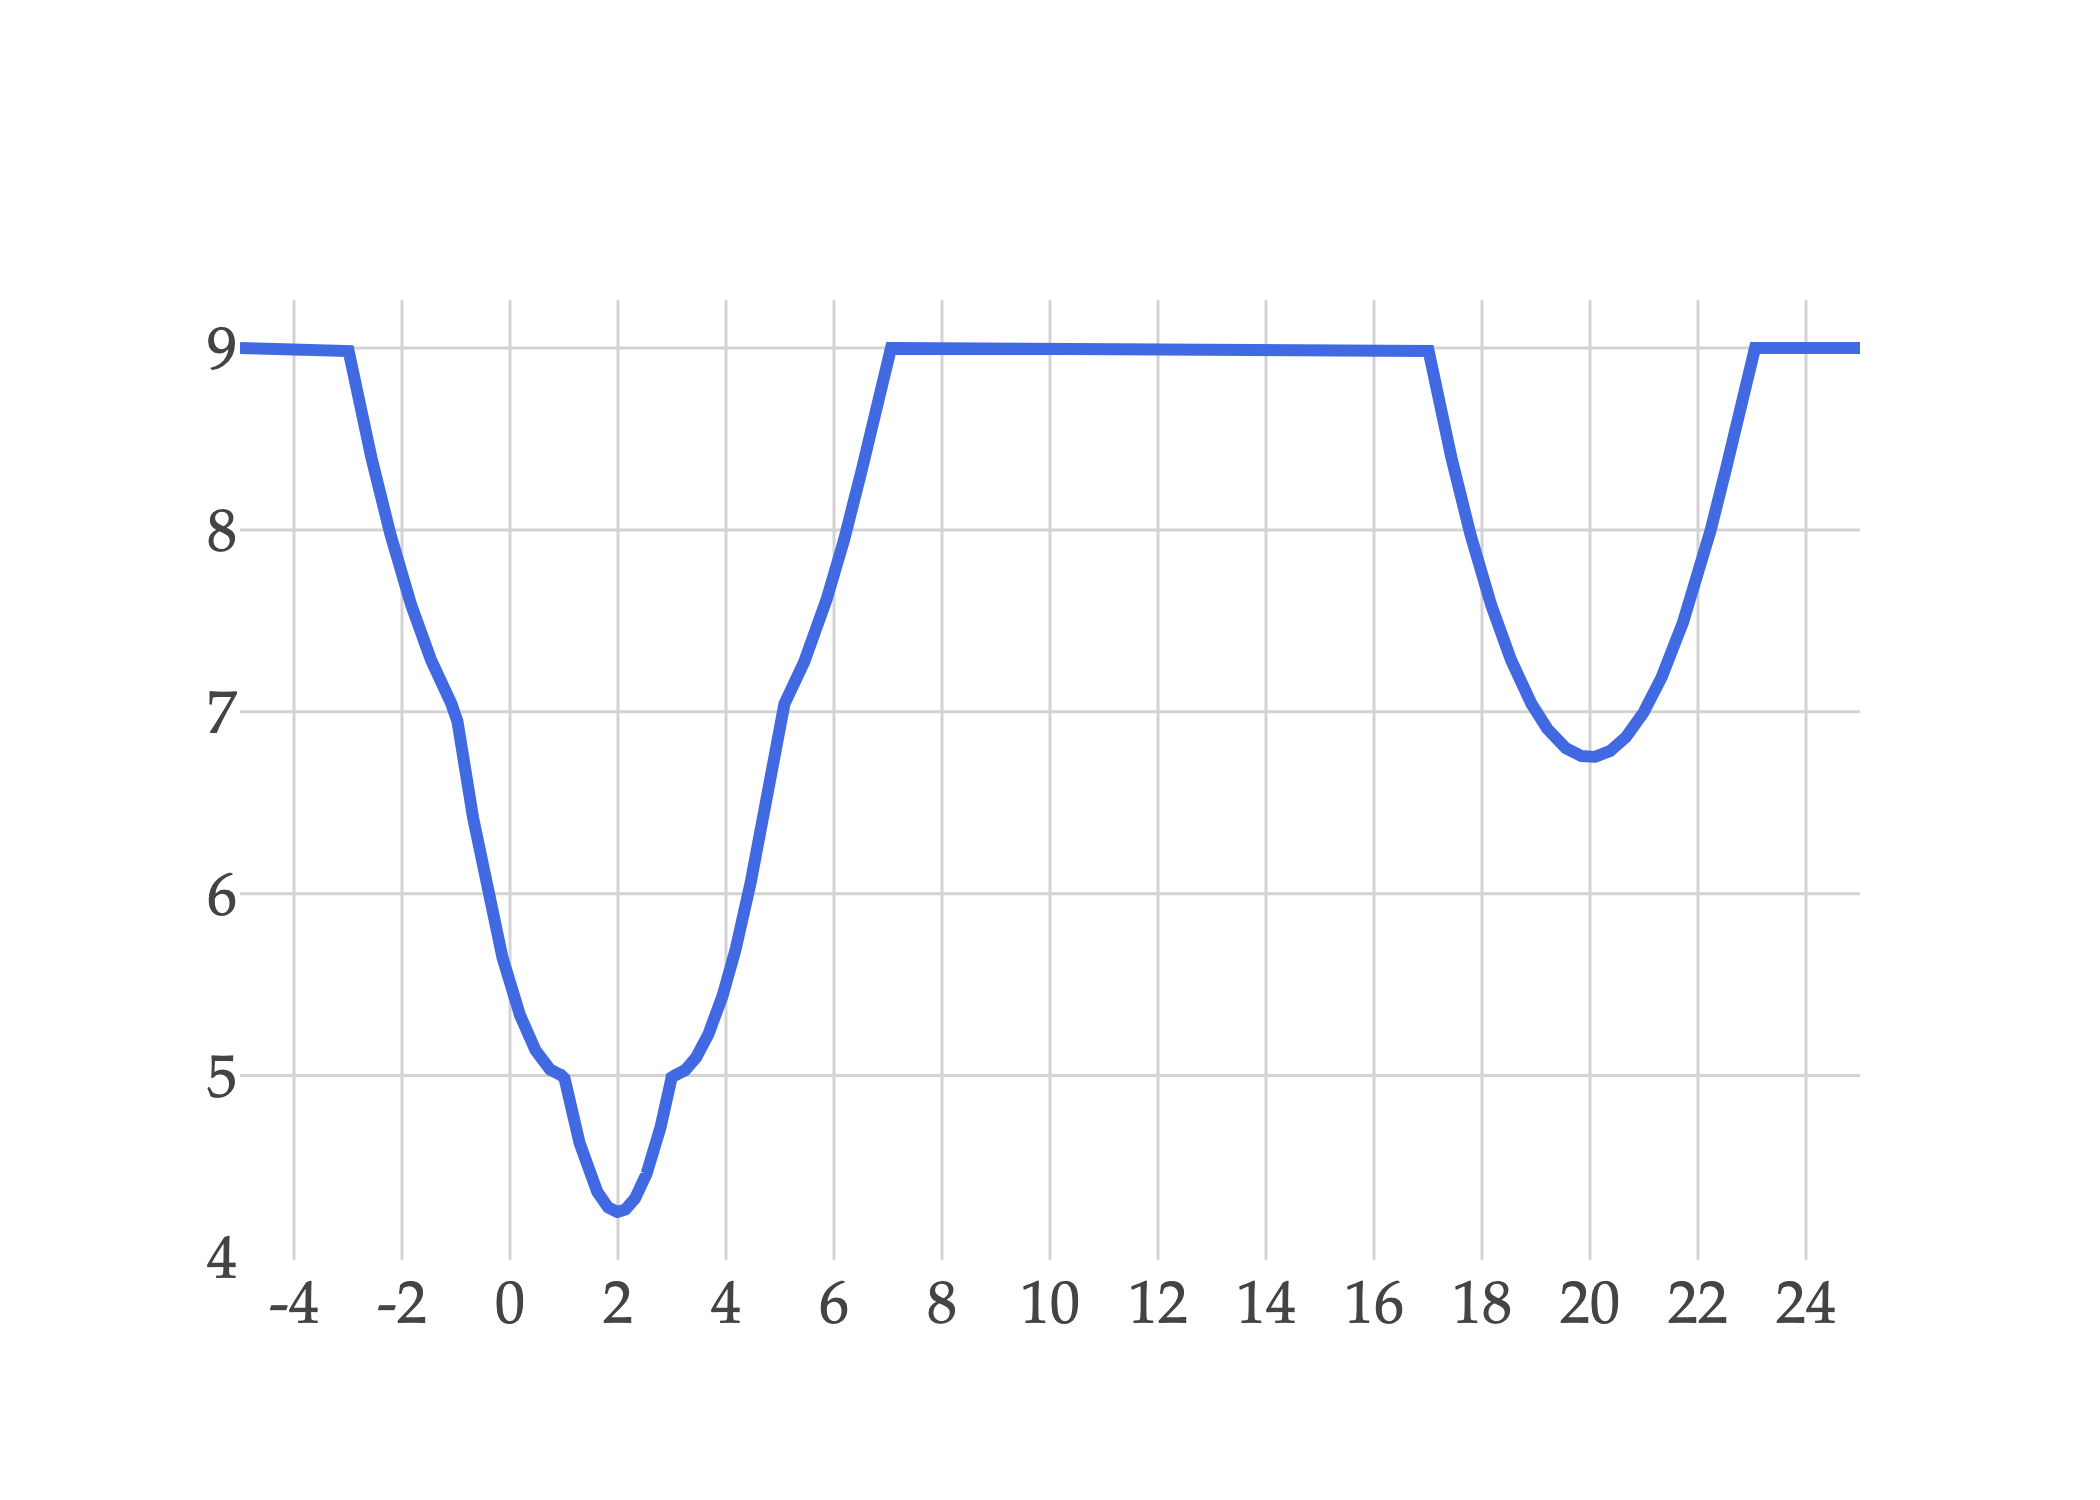
\includegraphics[width=0.9\textwidth]{imgs/p1-sol.png}
\end{center}

First, note that $w = 20$ is a local minimizer of $R_\text{clip}(w)$: if we zoom in to the graph of $R_\text{clip}(w)$ around $w = 20$, it looks like a parabola that opens up, centered at $w = 20$. But, when we zoom out, we see that the graph falls even lower near $w = 2$ than it does near $w = 20$. \\

Why is this? It's because there are many more $y_i$ values within 3 units of $w = 2$ than there are within 3 units of $w = 20$. Remembering that we have $y_1 = 0, y_2 = 2, y_3 = 4, y_4 = 20$:

$$R_\text{clip}(20) = \frac{1}{4} \sum_{i=1}^4 \min\{(20-y_i)^2, 9\} = \frac{1}{4} \left( 9 + 9 + 9 + 0 \right) = \frac{27}{4}$$
$$R_\text{clip}(2) = \frac{1}{4} \sum_{i=1}^4 \min\{(2-y_i)^2, 9\} = \frac{1}{4} \left( 4 + 0 + 4 + 9 \right) = \frac{17}{4}$$

So, $R_\text{clip}(20) = \frac{27}{4} > \frac{13}{4} = R_\text{clip}(2)$. \\

The question, then, is whether $w=2$ is the global minimizer, or just that it's better than $w=20$. Crucially, you wouldn't have had the graph of $R_\text{clip}(w)$ during the exam, so you would have needed to reason about this without it. One way to see how $w = 2$ is the global minimizer is to realize that as $w$ increases from $2$, the average loss only increases, until it reaches 9, where it ``coasts'' until it we reach $w = 17$, where it decreases once again.

\end{solution}
\end{subprob}

\begin{subprob}(4 pts) State one pro and one con of using clipped loss instead of squared loss to find optimal model parameters. \\
\emptybox{3cm}
\begin{solution}
One pro is that clipped loss is less sensitive to outliers, since very large errors all receive the same loss of $9$. One con is that it stops distinguishing between bad and very bad predictions once the error is large enough; it also introduces points where the derivative is not defined, when the two cases of the min function switch.
\end{solution}
\end{subprob}
\end{prob}

\newpage

\begin{prob}[(10 pts)]
We will continue to use the constant model, $h(x_i)=w$, and the same dataset of $n=4$ values as in Problem 1:
\[
0,\quad 2,\quad 4,\quad 20
\]
Instead of the clipped loss function, consider the \textbf{weighted absolute} loss function, defined below.
\[
L_\text{WA}(y_i,h(x_i))=
\begin{cases}
\beta(y_i-h(x_i)), & h(x_i)<y_i \\
h(x_i)-y_i, & h(x_i)\ge y_i
\end{cases}
\]
where $\beta$ is a positive integer. Let $R_\text{WA}(w)$ be the average weighted absolute loss for the constant model and this dataset.

The slope of $R_\text{WA}(w)$ at $w$, for any value of $w$ not equal to one of the $y_i$ values, is

$$\text{slope of } R_\text{WA}(w) \text{ at } w = \frac{\#\text{ left of } w - \beta(\#\text{ right of } w)}{4}$$

\begin{subprob}(4 pts) Suppose $\beta = 1$. Which value of $w$ minimizes $R_\text{WA}(w)$? Show your work, and write your final answer in the box provided. Your answer should be a number with no variables. If there are multiple possible answers, state just one. \\

\labeledanswerbox{\text{minimizer of } R_\text{WA}(w)}{3}[3cm][3cm][1cm]
\begin{solution}
When $\beta = 1$, $R_{\text{WA}}(w)$ is just mean absolute error, $R_\text{abs}(w)$. We know that the minimizer of mean absolute error is the median of the dataset, or any value between the middle two values if the dataset has an even number of values. \\

This dataset has an even number of values, so any $w$ in the interval $2 \leq w \leq 4$ minimizes $R_\text{WA}(w)$. One such value is $\boxed{3}$, but $2$, $4$, $\pi$, etc. are all valid answers.
\end{solution}
\end{subprob}

\begin{subprob}(6 pts) Now suppose $\beta = 2$. Which value of $w$ minimizes $R_\text{WA}(w)$? Show your work, and write your final answer in the box provided. Your answer should be a number with no variables. If there are multiple possible answers, state just one. \\

\labeledanswerbox{\text{minimizer of } R_\text{WA}(w)}{4}[7cm][3cm][1cm]
\begin{solution}
When $\beta=2$, the slopes between consecutive data values are
\[
-2,\quad -\frac54,\quad -\frac12,\quad \frac14,\quad 1
\]
on the intervals $(-\infty,0)$, $(0,2)$, $(2,4)$, $(4,20)$, and $(20,\infty)$. The slope changes from negative to positive at $w=4$, so the minimizer is $\boxed{4}$. \\

Conceptually, the fact that the errors in the case where $y_i > h(x_i)$ are multiplied by $\beta$ forces the optimal $w^*$ to be larger than the median (since we want the $y_i > h(x_i)$ case to not trigger as often when computing the average loss across the entire dataset).
\end{solution}
\end{subprob}

% \begin{subprob}(6 pts) Explain why

% \emptybox{8cm}

% \end{subprob}

% \begin{subprob}(XX pts) For a generic dataset and a generic fixed positive integer $\beta$, what is the minimizer of $R_\text{WA}(w)$? Describe it in one English sentence.

% \par\noindent\emptybox{2.2cm}
% \end{subprob}
\end{prob}

\newpage

\begin{prob}[(14 pts)]
Suppose we fit a simple linear regression model \textbf{with} an intercept term, $h(x_i)=w_0+w_1x_i$,
to a dataset of $n$ points $(x_1, y_1), (x_2, y_2), \ldots, (x_n, y_n)$ by minimizing mean squared error. You are given the following information:

\begin{itemize}
    \item The fit model satisfies $h(-4) = 5$ and $h(8) = 14$.
    \item The mean of $y_1, y_2, \ldots, y_n$ is $\bar y = 2$.
\end{itemize}

\begin{subprob}(6 pts) Find $\bar x$, the mean of $x_1, x_2, \ldots, x_n$. Show your work, and write your final answer in the box provided. Your answer should be a number with no variables. \textit{Hint: What property does the line $h(x_i)$ satisfy?} \\

\labeledanswerbox{\text{$\bar x$}}{$-8$}[12cm][3cm][1cm]

\begin{solution}
The line through $(-4,5)$ and $(8,14)$ has slope
\[
w_1^*=\frac{14-5}{8-(-4)}=\frac{9}{12}=\frac34
\]
Using $h(-4)=5$,
\[
5=w_0^*+\frac34(-4)=w_0^*-3
\]
so $w_0^*=8$, and the fit model is $h(x_i) = 8 + \frac{3}{4}x_i$. \\

For simple linear regression with an intercept, the fit line passes through $(\bar x,\bar y)$. Since $\bar y=2$,
\[
2=8+\frac34\bar x \implies \bar x = -8
\]
which gives $\boxed{\bar x=-8}$.
\end{solution}
\end{subprob}

\begin{subprob}(4 pts) Suppose the correlation coefficient between the $x$-values and $y$-values is $r = 1/3$.

The standard deviation of $y$, $\sigma_y$, is $c$ times the standard deviation of $x$, $\sigma_x$. In other words, $$\sigma_y = c \sigma_x$$ What is the value of $c$?

\bubble{$1/4$} \bubble{$4/9$} \bubble{$3/4$} \correctbubble{$9/4$} \bubble{$3$} \bubble{$4$}
\begin{solution}
For simple linear regression, one (of the many equivalent) formula for the slope $w_1^*$ is
\[
w_1^*=r\frac{\sigma_y}{\sigma_x}
\]
From part \textbf{a)}, $w_1^*=\frac34$. Since $r=\frac13$ and $\sigma_y=c\sigma_x$,
\[
\frac34=\frac13c
\]
so $\boxed{c=\frac94}$.
\end{solution}
\end{subprob}

\begin{subprob}(4 pts) Let $e_i=y_i-h(x_i)$ be the fit model's error for the $i$th point. Note that $e_i$ may either be positive or negative. Which of the following statements are \textbf{guaranteed} to be true? \textbf{Select all} that apply. \\

\correctsquarebubble{$\displaystyle\sum_{i=1}^n e_i=0$} \hspace{0.25in}
\correctsquarebubble{$\displaystyle\sum_{i=1}^n x_i e_i=0$} \hspace{0.25in}
\squarebubble{$\displaystyle\sum_{i=1}^n y_i e_i=0$} \hspace{0.25in}
\correctsquarebubble{$\displaystyle\sum_{i=1}^n e_i (x_i - \bar x)=0$}
\begin{solution}
How did we find $w_0^*$ and $w_1^*$? By minimizing mean squared error:

$$R_\text{sq}(w_0, w_1) = \frac{1}{n} \sum_{i=1}^n (y_i - (w_0 + w_1 x_i))^2$$

To do so, we took the partial derivatives with respect to $w_0$ and $w_1$ and set them equal to 0:
\[
\frac{\partial R_\text{sq}}{\partial w_0} = \frac{1}{n} \sum_{i=1}^n -2(y_i - (w_0 + w_1 x_i)) = 0
\]
\[
\frac{\partial R_\text{sq}}{\partial w_1} = \frac{1}{n} \sum_{i=1}^n -2x_i(y_i - (w_0 + w_1 x_i)) = 0
\]

Solving these equations gave us $w_0^*$ and $w_1^*$. But if we take a closer look, these equations are telling us properties about the errors, $e_i = y_i - h(x_i) = y_i - (w_0 + w_1 x_i)$. Above, I'll substitute in $e_i$ every time I see a $y_i - (w_0 + w_1 x_i)$. \\

The first equation becomes

$$\frac{1}{n} \sum_{i=1}^n -2e_i = 0 \implies \sum_{i=1}^n e_i = 0$$

and the second equation becomes

$$\frac{1}{n} \sum_{i=1}^n -2x_i e_i = 0 \implies \sum_{i=1}^n x_i e_i = 0$$

So, hidden in plain sight were these properties about the errors! Recall, the four options in this question are:
\begin{itemize}
  \item $\displaystyle\sum_{i=1}^n e_i=0$
  \item $\displaystyle\sum_{i=1}^n x_i e_i=0$
  \item $\displaystyle\sum_{i=1}^n y_i e_i=0$
  \item $\displaystyle\sum_{i=1}^n e_i(x_i-\bar x)=0$
\end{itemize}

So, we know the first two are true. \\

What about the third option, $\displaystyle\sum_{i=1}^n y_i e_i=0$? The short answer is that there's no reason to believe this is true; if it were, it would have emerged from our analysis above. To be sure that it's not true, let's find a counterexample.

We know that $y_i = h(x_i) + e_i$, so
\[
\sum_{i=1}^n y_i e_i = \sum_{i=1}^n (h(x_i) + e_i) e_i = \sum_{i=1}^n h(x_i) e_i + \sum_{i=1}^n e_i^2
\]

This is only $0$ when the fit line has zero error on every point. So, the third option is not guaranteed to be true. \\

Finally, let's look at the fourth option, $\sum_{i=1}^n e_i(x_i-\bar x)=0$. This is true, because the first two options are true:
\[
\sum_{i=1}^n e_i(x_i-\bar x)=\sum_{i=1}^n e_i x_i -\sum_{i=1}^n e_i \bar x = 0 - \bar x \sum_{i=1}^n e_i = 0
\]
The statement $\sum_{i=1}^n y_i e_i=0$ is not guaranteed; in fact, since $y_i=h(x_i)+e_i$,
\[
\sum_{i=1}^n y_i e_i=\sum_{i=1}^n h(x_i)e_i+\sum_{i=1}^n e_i^2=\sum_{i=1}^n e_i^2
\]
which is only $0$ when the fit line has zero error on every point, i.e. passes through every single point.

\textbf{Above, you may be wondering why it's the case that}

$$\sum_{i = 1}^n h(x_i) e_i = 0$$

Intentionally, I haven't provided the proof of this! I want you to piece the proof together. Start by using the fact that the first two options in this question are true.

\end{solution}
\end{subprob}
\end{prob}

\vspace{0.25in}

\begin{prob}[(8 pts)]
Let $\vec u,\vec v\in\mathbb R^n$ be vectors satisfying
\[
\|\vec v\|=5,\qquad \|\vec u+\vec v\|=10,\qquad \|\vec u-\vec v\|=6
\]

% \begin{subprob}(XX pts)
Find $\lVert \vec u \rVert^2$ (\textbf{not} $\lVert \vec u \rVert$). Show your work, and write your final answer in the box provided. Your answer should be a number with no variables.

\labeledanswerbox{\text{$\lVert \vec u \rVert^2$}}{$43$}[14.5cm][3cm][1cm]

\begin{solution}
We have
\[
10^2=\|\vec u+\vec v\|^2=\|\vec u\|^2+2\vec u\cdot\vec v+\|\vec v\|^2
\]
and
\[
6^2=\|\vec u-\vec v\|^2=\|\vec u\|^2-2\vec u\cdot\vec v+\|\vec v\|^2
\]
Notice that the expressions on the right-hand side are similar, except for the signs of $2 \vec u \cdot \vec v$. So, adding these equations gives
\[
136=2\|\vec u\|^2+2\|\vec v\|^2=2\|\vec u\|^2+50
\]
so

$$\lVert \vec u \rVert^2 = \frac{136 - 50}{2} = \boxed{43}$$
\end{solution}
% \end{subprob}

% \newpage

% \begin{subprob}(XX pts) Suppose $\vec p$ is the projection of $\vec u$ onto $\vec v$. Find $\lVert \vec p \rVert$. Show your work, and write your final answer in the box provided. Your answer should be a number with no variables. \\

% \labeledanswerbox{\text{$\lVert \vec p \rVert$}}{$16/5$}[14.5cm][3cm][1cm]

% \end{subprob}

% \begin{subprob}(XX pts) This part is independent of the previous parts. \\

% Suppose $\vec u, \vec v \in \mathbb{R}^n$, $\vec v\ne \vec 0$, and that $\lVert \vec u + \vec v \rVert = \lVert \vec u - \vec v \rVert$. True or False: The projection of $\vec u$ onto $\vec v$ is guaranteed to be $\vec 0$. \\

% \correctbubble{True} \bubble{False}

% \end{subprob}
\end{prob}

\newpage

\begin{prob}[(13 pts)]
Suppose $\vec u,\vec v\in\mathbb R^n$ are non-zero vectors and $k$ is a scalar. Let
$$f(k) = \lVert \vec u - k \vec v \rVert^2 + C k^2$$
where $C \geq 0$ is a non-negative constant.

\begin{subprob}(6 pts) In this part only, suppose $C=0$, $\vec u = \begin{bmatrix} 1 \\ 2 \end{bmatrix}$, and $\vec v = \begin{bmatrix} 3 \\ 1 \end{bmatrix}$. Find the value of $k$ that minimizes $f(k)$. Show your work, and write your final answer in the box provided. Your answer should be a number with no variables. \\

\labeledanswerbox{\text{minimizer of } f(k)}{1/2}[4cm][3cm][1cm]

\begin{solution}
There are several ways to think about this problem. What I expected most students to see is that when $C = 0$, this is really asking for the orthogonal projection of $\vec u$ onto $\vec v$; the minimizer of $f(k)$ is the value of $k$ that makes $\vec u - k \vec v$ orthogonal to $\vec v$. \\

Using that logic, we know from \href{https://notes.eecs245.org/vectors/orthogonal-projection/}{Chapter 3.4} that the orthogonal projection of $\vec u$ onto $\vec v$ is given by

$$\vec p = k^* \vec v = \left( \frac{\vec u \cdot \vec v}{\vec v \cdot \vec v} \right) \vec v$$

So, $$k^* = \frac{\vec u \cdot \vec v}{\vec v \cdot \vec v} = \frac{1 \cdot 3 + 2 \cdot 1}{3^2 + 1^2} = \frac{5}{10} = \boxed{\frac{1}{2}}$$

There's another way to approach this problem, which is to simplify $f(k)$ and treat this like a calculus problem. 
\[
f(k)=\left\|\begin{bmatrix}1\\2\end{bmatrix}-k\begin{bmatrix}3\\1\end{bmatrix}\right\|^2=(1-3k)^2+(2-k)^2
\]
Expanding,
\[
f(k)=10k^2-10k+5
\]
so
\[
f'(k)=20k-10
\]
Setting $f'(k)=0$ gives $k^* = \frac{1}{2}$ as well.
\end{solution}
\end{subprob}

% \begin{subprob}(XX pts) In general, for any $\vec u$, $\vec v$, and $C$, find the value of $k$ that minimizes $f(k)$. Show your work, and write your final answer in the box provided. Your answer should be an expression involving $\vec u$, $\vec v$, and/or $C$. \textit{Hint: You'll need to use calculus.}

% \labeledanswerbox{\text{minimizer of } f(k)}{TODO}[14.5cm][3cm][3cm]
% \end{subprob}

% \newpage
\begin{subprob}(4 pts) Note that $f(k)$ \textit{almost} looks like the squared norm of the vector $\vec u - k \vec v$, but with an extra term $C k^2$. Let's try and rewrite $f(k)$ so that it \textit{is} the squared norm of another related vector.

Define two new vectors, $\vec U, \vec V \in \mathbb R^{n+1}$ by appending the scalar $a$ to the end of $\vec u$ and the scalar $b$ to the end of $\vec v$.

$$\vec U = \begin{bmatrix} u_1 \\ u_2 \\ \vdots \\ u_n \\ a\end{bmatrix}, \quad \vec V = \begin{bmatrix} v_1 \\ v_2 \\ \vdots \\ v_n \\ b\end{bmatrix}$$

Select values of $a$ and $b$ so that $f(k) = \lVert \vec U - k \vec V \rVert^2$, for all possible non-negative values of $C$.

\begin{enumerate}[label=(\roman*)]
  \item What is the value of $a$? \correctbubble{0} \bubble{$C$} \bubble{$C^2$} \bubble{$\sqrt{C}$}
  \item What is the value of $b$? \bubble{0} \bubble{$C$} \bubble{$C^2$} \correctbubble{$\sqrt{C}$}
\end{enumerate}
\begin{solution}
First, let's try and get a better sense of how $\lVert \vec U - k \vec V \rVert^2$ works.

\begin{align*}
\lVert \vec U - k \vec V \rVert^2 &= \left\lVert \begin{bmatrix} u_1 \\ u_2 \\ \vdots \\ u_n \\ a\end{bmatrix} - k \begin{bmatrix} v_1 \\ v_2 \\ \vdots \\ v_n \\ b\end{bmatrix} \right\rVert^2 \\
&= \left\lVert \begin{bmatrix} u_1 - kv_1 \\ u_2 - kv_2 \\ \vdots \\ u_n - kv_n \\ a - kb\end{bmatrix} \right\rVert^2 \\
&= \sum_{i=1}^n (u_i - kv_i)^2 + (a - kb)^2 \\
&= \lVert \vec u - k \vec v \rVert^2 + (a - kb)^2 \\
\end{align*}

Our job is to find $a$ and $b$ so that $f(k)$, which we were told is defined as $$f(k) =\lVert \vec u - k \vec v \rVert^2 + C k^2$$ is \textbf{also} equal to $$\lVert \vec U - k \vec V \rVert^2 = \lVert \vec u - k \vec v \rVert^2 + (a - kb)^2$$

If we set $f(k) = \lVert \vec U - k \vec V \rVert^2$, we see that this boils down to finding $a$ and $b$ such that $$(a - kb)^2 = C k^2$$

Notice the right-hand side of the expression above is just $Ck^2$, not $Ck^2 + \text{some constant} \cdot k + \text{some other constant}$. This means that $a = 0$, and that forces $b = \sqrt{C}$:

$$(0 - k\sqrt{C})^2 = Ck^2$$

So, the correct answers are $\boxed{a=0}$ and $\boxed{b=\sqrt{C}}$.
\end{solution}
\end{subprob}

\begin{subprob}(3 pts) As $C$ increases, what happens to the value of $k$ that minimizes $f(k)$? Explain your reasoning. \\

\emptybox{3.5cm}

\begin{solution}
There are a couple of ways to think about this. First, if we use the interpretation provided in part \textbf{b)}, the vectors $\vec U$ and $\vec V$ ``bake in'' the value of $C$:

$$\vec U = \begin{bmatrix} u_1 \\ u_2 \\ \vdots \\ u_n \\ 0\end{bmatrix}, \quad \vec V = \begin{bmatrix} v_1 \\ v_2 \\ \vdots \\ v_n \\ \sqrt{C}\end{bmatrix}$$

Increasing $C$ keeps the dot product of $\vec U$ and $\vec V$ fixed, but increases the norm of $\vec V$. Why is this relevant? Since $f(k) = \lVert \vec U - k \vec V \rVert^2$, the minimizer $k^*$ of $f(k)$ is equal to

$$k^* = \frac{\vec U \cdot \vec V}{\vec V \cdot \vec V}$$

So, as $C$ increases, the denominator of $k^*$ increases, so $k^*$ moves toward $0$, though this may happen either from the left or the right, since $\vec U \cdot \vec V$ may be positive or negative. \\

If you'd prefer, you \textit{could} just expand the original definition of $f(k)$, take the derivative to find the closed-form expression for the minimizing $k^*$ for an arbitrary $C$, and look at what happens to $k^*$ as $C$ increases. \\

Recall, the original definition of $f(k)$ is $f(k)=\lVert \vec u - k \vec v \rVert^2 + C k^2$, so
\[
f(k)=\vec u \cdot \vec u - 2k(\vec u\cdot\vec v)+k^2\vec v \cdot \vec v+Ck^2
\]
Therefore,
\[
f'(k)=-2(\vec u\cdot\vec v)+2k(\vec v \cdot \vec v+C)
\]
so the minimizer is
\[
k^*=\frac{\vec u\cdot\vec v}{\vec v \cdot \vec v+C}
\]
As $C$ increases, the denominator increases (but $\vec u$ and $\vec v$ are fixed --- notice these are the original $\vec u, \vec v$, not the new $\vec U, \vec V$), so $k^*$ moves toward $0$.
\end{solution}
\end{subprob}

% \begin{subprob}(XX pts) Now let $\lambda\ge 0$ be arbitrary. Find the value of $k$ that minimizes $f(k)$ by expanding $f(k)$ as a quadratic in $k$ and differentiating.
% \par\noindent\emptybox{2.6cm}
% \end{subprob}

% \begin{subprob}(XX pts) Using part \textbf{b)}, describe the geometry: what point is projected, what line it is projected onto, and what the minimizing value of $k$ represents.
% \par\noindent\emptybox{1.6cm}
% \end{subprob}

% \begin{subprob}(XX pts) As $\lambda$ increases, what happens geometrically to the minimizing value of $k$? Briefly explain without recomputing any derivatives.
% \par\noindent\emptybox{1.1cm}
% \end{subprob}
\end{prob}

\newpage

\begin{prob}[(11 pts)]
Suppose $c \in \mathbb R$ is a constant and
\[
\vec u=\begin{bmatrix}3\\1\\c\end{bmatrix},
\qquad
\vec v=\begin{bmatrix}6\\c\\-2\end{bmatrix}
\]

\begin{subprob}(4 pts)
Fill in the blanks to complete the sentence:

\begin{center}For all values of $c$, $\text{span}(\{\vec u,\vec v\})$ is a \_\_(i)\_\_-dimensional subspace of \_\_(ii)\_\_.\end{center}

(i): \minibox{3cm}{2}[1cm] \hspace{0.5in} (ii): \minibox{3cm}{$\mathbb R^3$}[1cm]
\begin{solution}
The vectors $\vec u$ and $\vec v$ are never scalar multiples of each other. If $\vec v=\lambda\vec u$, then the first entries force $\lambda=2$, the second entries force $c=2$, and the third entries force $-2=2c=4$, which is impossible. Therefore, the span is always a 2-dimensional subspace of $\mathbb R^3$. \\

Why $\mathbb R^3$? Because both $\vec u$ and $\vec v$ live in $\mathbb R^3$, so their span must also live in $\mathbb R^3$.
\end{solution}
\end{subprob}

\begin{subprob}(7 pts) Suppose the plane spanned by $\vec u$ and $\vec v$ is
\[
ax+24y+3z=0
\]
where $a$ is also a constant. Find the value of $c$. Show your work in the space provided, and write your final answer in the box provided. Your answer should be a number with no variables. \\

\labeledanswerbox{c}{$3$}[13cm][3cm][1cm]

\begin{solution}
There are a few ways to approach this. The first way starts by using the fact that $\vec u$ and $\vec v$ lie in the plane, which gives us a system of two equations and two unknowns. Plugging in the coordinates of $\vec u$ into the plane gives us
\[
3a+24+3c=0 \implies a + 8 + c = 0
\]
and plugging in the coordinates of $\vec v$ into the plane gives us
\[
6a+24c-6=0 \implies a + 4c - 1 = 0
\]
Subtracting the simplified versions of the two equations gives us

$$(8 + c) - (4c - 1) = 0 \implies 9 - 3c = 0 \implies c = 3$$

Another way to approach this is to find the cross product of $\vec u$ and $\vec v$, and try and write it as a scalar multiple of the vector $\begin{bmatrix} a \\ 24 \\ 3 \end{bmatrix}$. 

$$\vec u \times \vec v = \begin{bmatrix} 3 \\ 1 \\ c \end{bmatrix} \times \begin{bmatrix} 6 \\ c \\ -2 \end{bmatrix} = \begin{bmatrix} 1 \cdot (-2) - c \cdot c \\ c \cdot 6 - 3 \cdot (-2) \\ 3 \cdot c - 1 \cdot 6 \end{bmatrix} = \begin{bmatrix} -2 - c^2 \\ 6c + 6 \\ 3c - 6 \end{bmatrix}$$

Strictly speaking, this vector, $\begin{bmatrix} -2 - c^2 \\ 6c + 6 \\ 3c - 6 \end{bmatrix}$, is a scalar multiple of $\begin{bmatrix} a \\ 24 \\ 3 \end{bmatrix}$, but we don't know what the scalar is yet. So, we really should try and solve

$$\begin{bmatrix} -2 - c^2 \\ 6c + 6 \\ 3c - 6 \end{bmatrix} = k \begin{bmatrix} a \\ 24 \\ 3 \end{bmatrix}$$

But, notice that $6c + 6 = 24 \implies c = 3$, and $c = 3$ also satisfies $3c - 6 = 3$, so the scalar $k = 1$, and thus $\boxed{c = 3}$.

\end{solution}
\end{subprob}


\end{prob}

\newpage

\newpage

\begin{prob}[(10 pts)]
Suppose $\vec v_1,\vec v_2,\vec v_3,\vec v_4\in\mathbb R^n$ are a \textbf{linearly independent} collection of vectors. Define
\[
\vec p=\vec v_1+\vec v_2,\qquad
\vec q=\vec v_2+\vec v_3,\qquad
\vec r=\vec v_3+\vec v_4,\qquad
\vec s=\vec v_4+\vec v_1
\]

\begin{subprob}(7 pts) Are $\{\vec p,\vec q,\vec r,\vec s\}$ linearly independent?

\begin{enumerate}[label=(\roman*)]
    \item Select an answer: \bubble{Yes} \correctbubble{No}
    \item Prove your answer using the formal definition of linear independence. \textit{Hint: You did something similar in Homework 4, Problem 6.} \\
    \emptybox{14cm}
\end{enumerate}

\begin{solution}
If $\vec p,\vec q,\vec r,\vec s$ are linearly independent, then the only solution to the equation $a \vec p + b \vec q + c \vec r + d \vec s = \vec 0$ is $a = b = c = d = 0$. \\

That's not the case here! Consider the linear combination
\[
\vec p-\vec q+\vec r-\vec s
\]
How did I think of this? I noticed that if I start with $\vec p$, subtracting $\vec q$ gets rid of all $\vec v_2$'s, but makes $\vec v_3$ negative, so I need a positive $\vec r$ to cancel that out. Then, $\vec p - \vec q + \vec r = \vec v_1 + \vec v_4$; subtracting $\vec s$ then gets rid of both $\vec v_1$ and $\vec v_4$, leaving me with $\vec 0$. \\
\[
\vec p - \vec q + \vec r - \vec s = (\vec v_1+\vec v_2)-(\vec v_2+\vec v_3)+(\vec v_3+\vec v_4)-(\vec v_4+\vec v_1)=\vec 0
\]
The coefficients $1,-1,1,-1$ are not all zero, so this proves that $\{\vec p,\vec q,\vec r,\vec s\}$ is linearly dependent.
\end{solution}
\end{subprob}

\begin{subprob}(3 pts) What is the dimension of $\text{span}(\{\vec p,\vec q,\vec r,\vec s\})$? Give your answer as a number with no variables. \\

$\dim(\text{span}(\{\vec p,\vec q,\vec r,\vec s\})) = \minibox{3cm}{3}[1cm]$

\begin{solution}
Part \textbf{a)} shows that the four vectors are linearly \textbf{dependent}, so the dimension of $\text{span}(\{\vec p,\vec q,\vec r,\vec s\})$ is \textbf{at most} $3$. (For the dimension to be 4, which is the number of vectors in question, they would need to be linearly independent. There's no way to have a span of 5 or more dimensions using just 4 vectors.) \\

But just because the dimension of $\text{span}(\{\vec p,\vec q,\vec r,\vec s\})$ is at most $3$ doesn't mean that the dimension is actually $3$ --- for this span to be 3-dimensional, it needs to be the span of 3 linearly independent vectors. \\

Fortunately, $\vec p,\vec q,\vec r$ are linearly independent. If
\[
a\vec p+b\vec q+c\vec r=\vec 0
\]
then
\[
a\vec v_1+(a+b)\vec v_2+(b+c)\vec v_3+c\vec v_4=\vec 0
\]
Since $\vec v_1,\vec v_2,\vec v_3,\vec v_4$ are linearly independent, we must have
\[
a=0,\qquad a+b=0,\qquad b+c=0,\qquad c=0
\]
This gives $a=b=c=0$, so $\vec p,\vec q,\vec r$ are linearly independent. Therefore, among $\left\{ \vec p,\vec q,\vec r,\vec s \right\}$, there are 3 linearly independent vectors, and thus

$$\boxed{\dim(\text{span}(\{\vec p,\vec q,\vec r,\vec s\}))=3}$$
\end{solution}
\end{subprob}

% \begin{subprob}(XX pts) True or False: $\{\vec p,\vec q,\vec r,\vec v_4\}$ is a basis for $\text{span}(\{\vec v_1,\vec v_2,\vec v_3,\vec v_4\})$.

% \correctbubble{True} \bubble{False}

% \end{subprob}
\end{prob}

\newpage

\begin{prob}[(8 pts)]
Suppose $S$ is the subspace of $\mathbb R^4$ defined by
\[
S=\left\{
\begin{bmatrix}x_1\\x_2\\x_3\\x_4\end{bmatrix}\in\mathbb R^4 :
x_1-x_2+x_3-x_4=0
\right\}
\]

Which of the following sets is a basis for $S$? \textbf{Select all} that apply.

\correctsquarebubble{$\left\{
\begin{bmatrix}1\\1\\0\\0\end{bmatrix},
\begin{bmatrix}0\\1\\1\\0\end{bmatrix},
\begin{bmatrix}0\\0\\1\\1\end{bmatrix}
\right\}$}

\squarebubble{$\left\{
\begin{bmatrix}1\\1\\0\\0\end{bmatrix},
\begin{bmatrix}0\\1\\1\\0\end{bmatrix},
\begin{bmatrix}0\\0\\1\\1\end{bmatrix},
\begin{bmatrix}1\\0\\0\\1\end{bmatrix}
\right\}$}

\correctsquarebubble{$\left\{
\begin{bmatrix}1\\0\\0\\1\end{bmatrix},
\begin{bmatrix}0\\1\\0\\-1\end{bmatrix},
\begin{bmatrix}0\\0\\1\\1\end{bmatrix}
\right\}$}

% \squarebubble{$\left\{
% \begin{bmatrix}1\\1\\0\\0\end{bmatrix},
% \begin{bmatrix}0\\1\\1\\0\end{bmatrix},
% \begin{bmatrix}0\\0\\1\\1\end{bmatrix},
% \begin{bmatrix}0\\0\\2\\2\end{bmatrix}
% \right\}$}

\squarebubble{$\left\{
\begin{bmatrix}1\\0\\0\\1\end{bmatrix},
\begin{bmatrix}0\\1\\0\\-1\end{bmatrix},
\begin{bmatrix}1\\1\\0\\0\end{bmatrix}
\right\}$}

% For each of the following sets, identify whether or not it is a basis for $S$ and explain why.

  % \begin{subprob}(XX pts)

  % \begin{minipage}[t]{0.3\linewidth}
  % \vspace{0pt}
  % $\left\{
  % \begin{bmatrix}1\\1\\0\\0\end{bmatrix},
  % \begin{bmatrix}0\\1\\1\\0\end{bmatrix},
  % \begin{bmatrix}0\\0\\1\\1\end{bmatrix}
  % \right\}$
  % \end{minipage}\hfill\begin{minipage}[t]{0.65\linewidth}
  % \vspace{0pt}
  % \begin{enumerate}[label=(\roman*), topsep=0pt, itemsep=0.1em, parsep=0pt, partopsep=0pt]
  %     \item Basis for $S$? \bubble{Yes} \bubble{No}
  %     \item Justify your answer.

  %     \emptybox[\dimexpr\linewidth-2\fboxsep-2\fboxrule\relax]{3.2cm}
  % \end{enumerate}
  % \end{minipage}
  % \end{subprob}

% \begin{subprob}(XX pts)

% \begin{minipage}[t]{0.3\linewidth}
% \vspace{0pt}
% $\left\{
% \begin{bmatrix}1\\1\\0\\0\end{bmatrix},
% \begin{bmatrix}0\\1\\1\\0\end{bmatrix},
% \begin{bmatrix}0\\0\\1\\1\end{bmatrix},
% \begin{bmatrix}1\\0\\0\\1\end{bmatrix}
% \right\}$
% \end{minipage}\hfill\begin{minipage}[t]{0.65\linewidth}
% \vspace{0pt}
% \begin{enumerate}[label=(\roman*), topsep=0pt, itemsep=0.1em, parsep=0pt, partopsep=0pt]
%     \item Basis for $S$? \bubble{Yes} \bubble{No}
%     \item Justify your answer.

%     \emptybox[\dimexpr\linewidth-2\fboxsep-2\fboxrule\relax]{3.2cm}
% \end{enumerate}
% \end{minipage}
% \end{subprob}

% \begin{subprob}(XX pts)

% \begin{minipage}[t]{0.3\linewidth}
% \vspace{0pt}
% $\left\{
% \begin{bmatrix}1\\0\\0\\1\end{bmatrix},
% \begin{bmatrix}0\\1\\0\\-1\end{bmatrix},
% \begin{bmatrix}0\\0\\1\\1\end{bmatrix}
% \right\}$
% \end{minipage}\hfill\begin{minipage}[t]{0.65\linewidth}
% \vspace{0pt}
% \begin{enumerate}[label=(\roman*), topsep=0pt, itemsep=0.1em, parsep=0pt, partopsep=0pt]
%     \item Basis for $S$? \bubble{Yes} \bubble{No}
%     \item Justify your answer.

%     \emptybox[\dimexpr\linewidth-2\fboxsep-2\fboxrule\relax]{3.2cm}
% \end{enumerate}
% \end{minipage}
% \end{subprob}

% \begin{subprob}(XX pts)

% \begin{minipage}[t]{0.3\linewidth}
% \vspace{0pt}
% $\left\{
% \begin{bmatrix}1\\0\\0\\1\end{bmatrix},
% \begin{bmatrix}0\\1\\0\\-1\end{bmatrix},
% \begin{bmatrix}1\\1\\0\\0\end{bmatrix}
% \right\}$
% \end{minipage}\hfill\begin{minipage}[t]{0.65\linewidth}
% \vspace{0pt}
% \begin{enumerate}[label=(\roman*), topsep=0pt, itemsep=0.1em, parsep=0pt, partopsep=0pt]
%     \item Basis for $S$? \bubble{Yes} \bubble{No}
%     \item Justify your answer.

%     \emptybox[\dimexpr\linewidth-2\fboxsep-2\fboxrule\relax]{3.2cm}
% \end{enumerate}
% \end{minipage}
% \end{subprob}

\begin{solution}
The subspace $S$ has dimension $3$ because the single constraint lets us solve
\[
x_4=x_1-x_2+x_3
\]
This means that components 1, 2, and 3 are free to vary, and component 4 is fully determined by those first three components. So, $S$ has three ``degrees of freedom'', and therefore has dimension $3$. \\

So a basis for $S$ is any set of \textbf{three linearly independent vectors} that all lie in $S$. \\

The first and third choices are bases: in both of those choices, the set has 3 vectors that are linearly independent, and all 3 vectors lie in $S$. \\

The second choice has 4 vectors in a 3-dimensional subspace, so it cannot be a basis. \\

The fourth choice has 3 vectors but they are not linearly independent, since at least one of them can be written as a linear combination of the other two:
\[
\begin{bmatrix}1\\1\\0\\0\end{bmatrix} = \begin{bmatrix}1\\0\\0\\1\end{bmatrix} + \begin{bmatrix}0\\1\\0\\-1\end{bmatrix}
\]

So, only the first and third choices are bases for $S$.

\end{solution}
\end{prob}

\newpage

\begin{prob}[(10 pts)]
\begin{subprob}(7 pts) Suppose $x$ and $y$ are non-negative numbers. Using the Cauchy-Schwarz inequality, prove that
\[
\frac{(x+y)^2}{2}\le x^2+y^2
\]

\textit{Solutions that do not use the Cauchy-Schwarz inequality will not receive credit.}

\par\noindent\emptybox{12cm}
\begin{solution}
Recall, the Cauchy-Schwarz inequality states that for any two vectors $\vec u, \vec v \in \mathbb{R}^n$,
\[
|\vec u \cdot \vec v| \leq \|\vec u\| \|\vec v\|
\]

Applying Cauchy-Schwarz to the vectors $\vec u=\begin{bmatrix}x\\y\end{bmatrix}$ and $\vec v=\begin{bmatrix}1\\1\end{bmatrix}$ gives
\[
|x + y| \leq \sqrt{x^2 + y^2} \sqrt{1^2 + 1^2} = \sqrt{2(x^2 + y^2)}
\]
Squaring both sides gives
\[
(x + y)^2 \leq 2(x^2 + y^2)
\]
and finally, dividing both sides by $2$ gives
\[
\frac{(x+y)^2}{2}\le x^2+y^2
\]
as needed.
\end{solution}
\end{subprob}

\begin{subprob}(3 pts) Now suppose $x$, $y$, and $z$ are non-negative numbers. Which inequality is guaranteed to be true? \\

\begin{tabular}{@{}l@{}}
\bubble{$\displaystyle \frac{(x+y+z)^2}{2}\le x^2+y^2+z^2$} \\ \vspace{0.1in}
\correctbubble{$\displaystyle \frac{(x+y+z)^2}{3}\le x^2+y^2+z^2$} \\ \vspace{0.1in}
\bubble{$\displaystyle \frac{(x+y+z)^2}{2}\le x^3+y^3+z^3$} \\ \vspace{0.1in}
\bubble{$\displaystyle \frac{(x+y+z)^3}{3}\le x^3+y^3+z^3$} \\
\bubble{None of the above}
\end{tabular}

\begin{solution}
The Cauchy-Schwarz inequality directly implies one of the options, and the other options are all not guaranteed to be true. Extending our argument from part \textbf{a)}, let's now apply Cauchy-Schwarz to the vectors $\vec u=\begin{bmatrix}x\\y\\z\end{bmatrix}$ and $\vec v=\begin{bmatrix}1\\1\\1\end{bmatrix}$. This gives
\[
|x+y+z|\le \sqrt{x^2+y^2+z^2} \sqrt{1^2+1^2+1^2} = \sqrt{3(x^2+y^2+z^2)}
\]
Squaring both sides and dividing by $3$ gives
\[
\frac{(x+y+z)^2}{3}\le x^2+y^2+z^2
\]
which is the second option.
\end{solution}
\end{subprob}
\end{prob}

\iffalse
Moved to Spring 2026 Final brainstorming.

\begin{prob}[(XX pts)]
Suppose $S$ is a 4-dimensional subspace of $\mathbb R^7$, and
$\{\vec u_1,\vec u_2,\vec u_3,\vec u_4\}$ is a basis for $S$.
Also suppose $\vec z\in\mathbb R^7$ and $\vec z\notin S$.

For each statement below, determine whether it is True or False. If True, give a
short justification. If False, give a counterexample or a short explanation.

\begin{subprob}(XX pts) The set $\{\vec u_1,\vec u_2,\vec u_3,\vec z\}$ is linearly independent.

\correctbubble{True} \bubble{False}

\par\noindent\emptybox{2.5cm}
\end{subprob}

\begin{subprob}(XX pts) Any four nonzero vectors in $S$ form a basis for $S$.

\bubble{True} \correctbubble{False}

\par\noindent\emptybox{2.2cm}
\end{subprob}

\begin{subprob}(XX pts) Any five vectors in $S$ are linearly dependent.

\correctbubble{True} \bubble{False}

\par\noindent\emptybox{2.2cm}
\end{subprob}

\begin{subprob}(XX pts) $\dim(\text{span}(\{\vec u_1,\vec u_2,\vec u_3,\vec u_4,\vec z\}))=5$.

\correctbubble{True} \bubble{False}

\par\noindent\emptybox{2.5cm}
\end{subprob}
\end{prob}
\fi

\newpage

Congrats on finishing Midterm 1! Feel free to draw us a picture about EECS 245 in the box below.

\emptybox{20cm}

% Did you notice any violations of the Honor Code during the exam? If so, share details with us here. We will keep your identity anonymous when investigating any cases.

% \emptybox{3cm}

\end{document}
